\documentclass[11pt]{article}
\usepackage{amsmath,amsthm,amssymb}
\usepackage[colorlinks]{hyperref}
\usepackage{tikz, pgfplots}
\pgfplotsset{compat=1.17}

\begin{document}
\title{Quick answer key to Recitation 10}
\author{ChatGPT 4o}
\date{7 October 2024}
\maketitle

Use the table of contents below to skip to a specific part
without seeing spoilers to the other parts.

I just used ChatGPT to write this one quickly.
ChatGPT can make mistakes, so if you spot anything that's wrong, flag me to ask.

\tableofcontents



\newpage

\section{Solution}

We are given the function \( f(x, y) = \frac{1}{x^2 + y^2} \). We will go through each part of the question step by step.

\subsection{Part 1: Draw the level curves for \( f(x, y) = 1 \) and \( f(x, y) = 2 \)}

The level curves for the function are obtained by setting \( f(x, y) = c \) for some constant \( c \), i.e.:
\[
f(x, y) = \frac{1}{x^2 + y^2} = c
\]
\[
x^2 + y^2 = \frac{1}{c}
\]

For \( f(x, y) = 1 \), we have:
\[
x^2 + y^2 = 1
\]
This is the equation of a circle with radius 1.

For \( f(x, y) = 2 \), we have:
\[
x^2 + y^2 = \frac{1}{2}
\]
This is the equation of a circle with radius \( \frac{1}{\sqrt{2}} \).

The level curves are circles centered at the origin with different radii. Below is the plot of the level curves:

\begin{center}
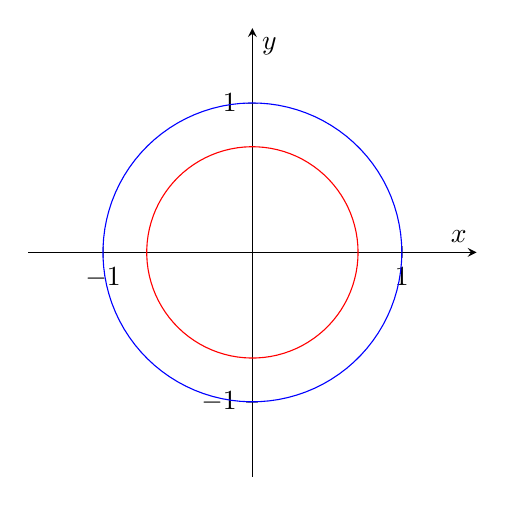
\begin{tikzpicture}
    \begin{axis}[
        axis lines = middle,
        xlabel = $x$, ylabel = $y$,
        xmin = -1.5, xmax = 1.5,
        ymin = -1.5, ymax = 1.5,
        axis equal image
    ]
    \addplot[domain=0:2*pi,samples=100,blue] ({cos(deg(x))}, {sin(deg(x))});
    \addplot[domain=0:2*pi,samples=100,red] ({cos(deg(x))/sqrt(2)}, {sin(deg(x))/sqrt(2)});
    \end{axis}
\end{tikzpicture}
\end{center}

The blue circle represents the level curve for \( f(x, y) = 1 \), and the red circle represents the level curve for \( f(x, y) = 2 \).

\newpage

\subsection{Part 2: Sketch the graph of \( f(x, y) \)}

The function \( f(x, y) = \frac{1}{x^2 + y^2} \) is a surface that decreases as \( x^2 + y^2 \) increases. The surface is radially symmetric and decreases toward 0 as we move away from the origin.

See WolframAlpha for a picture.

%Here is a 3D sketch of the graph:
%
%\begin{center}
%\begin{tikzpicture}
%    \begin{axis}[
%        view={60}{30},
%        xlabel = $x$, ylabel = $y$, zlabel = $f(x, y)$,
%        domain = -2:2,
%        samples = 50,
%        zmin = 0, zmax = 2,
%        colormap/viridis
%    ]
%    \addplot3[surf, shader=interp] {1/(x^2 + y^2)};
%    \end{axis}
%\end{tikzpicture}
%\end{center}

\newpage

\subsection{Part 3: Find the partial derivatives \( f_x(x, y) \) and \( f_y(x, y) \)}

The partial derivative of \( f(x, y) \) with respect to \( x \) is:
\[
f_x(x, y) = \frac{\partial}{\partial x} \left( \frac{1}{x^2 + y^2} \right)
\]
Using the chain rule:
\[
f_x(x, y) = -\frac{1}{(x^2 + y^2)^2} \cdot 2x = -\frac{2x}{(x^2 + y^2)^2}
\]

Similarly, the partial derivative with respect to \( y \) is:
\[
f_y(x, y) = \frac{\partial}{\partial y} \left( \frac{1}{x^2 + y^2} \right) = -\frac{2y}{(x^2 + y^2)^2}
\]

Thus, the partial derivatives are:
\[
f_x(x, y) = -\frac{2x}{(x^2 + y^2)^2}, \quad f_y(x, y) = -\frac{2y}{(x^2 + y^2)^2}
\]

\newpage

\subsection{Part 4: In what direction does \( f(x, y) \) increase the fastest at \( (1, 2) \)? What is the rate of increase in this direction?}

The direction in which \( f(x, y) \) increases the fastest is given by the gradient of \( f(x, y) \):
\[
\nabla f(x, y) = \left\langle f_x(x, y), f_y(x, y) \right\rangle
\]
At the point \( (1, 2) \), the gradient is:
\[
\nabla f(1, 2) = \left\langle -\frac{2(1)}{(1^2 + 2^2)^2}, -\frac{2(2)}{(1^2 + 2^2)^2} \right\rangle = \left\langle -\frac{2}{25}, -\frac{4}{25} \right\rangle
\]

To get the unit vector direction \( \mathbf{u} \) in which \( f(x, y) \) increases the fastest, we normalize the gradient vector:
\[
\mathbf{u} = \frac{\nabla f(1, 2)}{|\nabla f(1, 2)|} = \frac{1}{\sqrt{\left( -\frac{2}{25} \right)^2 + \left( -\frac{4}{25} \right)^2}} \left\langle -\frac{2}{25}, -\frac{4}{25} \right\rangle
\]
\[
= \frac{25}{5} \left\langle -\frac{2}{25}, -\frac{4}{25} \right\rangle = \left\langle -\frac{2}{5}, -\frac{4}{5} \right\rangle
\]

The rate of increase in this direction is the magnitude of the gradient:
\[
|\nabla f(1, 2)| = \sqrt{\left( -\frac{2}{25} \right)^2 + \left( -\frac{4}{25} \right)^2} = \frac{1}{5}
\]

Thus, the rate of increase in this direction is \( \frac{1}{5} \).

\newpage

\subsection{Part 5: Find the directional derivative \( D_{\mathbf{u}}f(1, 2) \) for the unit vector \( \mathbf{u} = \left\langle \frac{1}{\sqrt{5}}, -\frac{2}{\sqrt{5}} \right\rangle \)}

The directional derivative in the direction of a unit vector \( \mathbf{u} = \left\langle u_1, u_2 \right\rangle \) is given by:
\[
D_{\mathbf{u}}f(x, y) = \nabla f(x, y) \cdot \mathbf{u} = f_x(x, y) u_1 + f_y(x, y) u_2
\]
At \( (1, 2) \), we have:
\[
D_{\mathbf{u}}f(1, 2) = \left( -\frac{2}{25} \right) \left( \frac{1}{\sqrt{5}} \right) + \left( -\frac{4}{25} \right) \left( -\frac{2}{\sqrt{5}} \right)
\]
\[
= -\frac{2}{25\sqrt{5}} + \frac{8}{25\sqrt{5}} = \frac{6}{25\sqrt{5}}
\]

Thus, the directional derivative is:
\[
D_{\mathbf{u}}f(1, 2) = \frac{6}{25\sqrt{5}}
\]




\newpage

\section{Solution}

We are tasked with estimating the value of \( \log(0.49^2 + 0.76) \) using the linear approximation of the function \( f(x, y) = \log(x^2 + y) \) near the point \( (x_0, y_0) = (0.5, 0.75) \).

\newpage

\subsection{Step 1: Compute the function value at \( (0.5, 0.75) \)}

The function is \( f(x, y) = \log(x^2 + y) \). At the point \( (x_0, y_0) = (0.5, 0.75) \):
\[
f(0.5, 0.75) = \log(0.5^2 + 0.75) = \log(0.25 + 0.75) = \log(1) = 0.
\]

\newpage

\subsection{Step 2: Compute the partial derivatives of \( f(x, y) \)}

The partial derivatives of \( f(x, y) = \log(x^2 + y) \) are:

\[
f_x(x, y) = \frac{\partial}{\partial x} \left( \log(x^2 + y) \right) = \frac{1}{x^2 + y} \cdot \frac{\partial}{\partial x} (x^2 + y) = \frac{2x}{x^2 + y},
\]
\[
f_y(x, y) = \frac{\partial}{\partial y} \left( \log(x^2 + y) \right) = \frac{1}{x^2 + y} \cdot \frac{\partial}{\partial y} (x^2 + y) = \frac{1}{x^2 + y}.
\]

\newpage

\subsection{Step 3: Evaluate the partial derivatives at \( (0.5, 0.75) \)}

Now, we evaluate the partial derivatives at the point \( (0.5, 0.75) \):
\[
f_x(0.5, 0.75) = \frac{2(0.5)}{0.5^2 + 0.75} = \frac{1}{1} = 1,
\]
\[
f_y(0.5, 0.75) = \frac{1}{0.5^2 + 0.75} = \frac{1}{1} = 1.
\]

\newpage

\subsection{Step 4: Use the linear approximation formula}

The linear approximation of the function \( f(x, y) \) near the point \( (x_0, y_0) = (0.5, 0.75) \) is given by:
\[
f(x, y) \approx f(x_0, y_0) + f_x(x_0, y_0)(x - x_0) + f_y(x_0, y_0)(y - y_0).
\]
Using the values we have calculated:
\[
f(x, y) \approx 0 + 1(x - 0.5) + 1(y - 0.75).
\]
Thus, the linear approximation is:
\[
f(x, y) \approx (x - 0.5) + (y - 0.75).
\]

\newpage

\subsection{Step 5: Apply the approximation to \( (x, y) = (0.49, 0.76) \)}

We now use the linear approximation to estimate \( f(0.49, 0.76) \):
\[
f(0.49, 0.76) \approx (0.49 - 0.5) + (0.76 - 0.75) = -0.01 + 0.01 = 0.
\]

\newpage

\subsection{Final Estimate}

Using the linear approximation, we estimate that:
\[
\log(0.49^2 + 0.76) \approx 0.
\]

Thus, the value of \( \log(0.49^2 + 0.76) \) is approximately 0 based on the linear approximation.





\newpage

\section{Solution}

We are given the surface \( S \) defined by the equation:
\[
xy - 2xz^2 + 3y^2z = 2
\]
This defines a level surface for the function \( f(x, y, z) = xy - 2xz^2 + 3y^2z \), with the equation \( f(x, y, z) = 2 \). We are asked to find the directional derivative of \( f(x, y, z) \) at the point \( (1, 1, 1) \) in the direction of a vector \( \mathbf{u} \) that is tangent to the surface \( S \) at this point. Additionally, we are asked to find the equation of the tangent plane to \( S \) at the point \( (1, 1, 1) \).

\subsection{Part 1: Directional Derivative in the Direction of a Tangent Vector}

To find the directional derivative of \( f(x, y, z) \) at the point \( (1, 1, 1) \) in the direction of a tangent vector \( \mathbf{u} \), we first compute the gradient of \( f(x, y, z) \). The gradient of \( f \) is:
\[
\nabla f(x, y, z) = \left\langle \frac{\partial f}{\partial x}, \frac{\partial f}{\partial y}, \frac{\partial f}{\partial z} \right\rangle
\]
We compute each partial derivative:
\[
\frac{\partial f}{\partial x} = y - 2z^2,
\]
\[
\frac{\partial f}{\partial y} = x + 6yz,
\]
\[
\frac{\partial f}{\partial z} = -4xz + 3y^2.
\]

Now, evaluate the gradient at the point \( (1, 1, 1) \):
\[
\nabla f(1, 1, 1) = \left\langle 1 - 2(1)^2, 1 + 6(1)(1), -4(1)(1) + 3(1)^2 \right\rangle = \langle -1, 7, -1 \rangle.
\]

Let \( \mathbf{u} \) be any vector tangent to the surface \( S \) at the point \( (1, 1, 1) \). Since \( \mathbf{u} \) is tangent to the surface, it must be perpendicular to the gradient \( \nabla f(1, 1, 1) \). Therefore, the dot product between \( \mathbf{u} \) and \( \nabla f(1, 1, 1) \) is:
\[
\nabla f(1, 1, 1) \cdot \mathbf{u} = 0.
\]

Since the directional derivative of \( f(x, y, z) \) in the direction of a vector tangent to the surface is the dot product of the gradient and the tangent vector, the directional derivative in the direction of \( \mathbf{u} \) is:
\[
D_{\mathbf{u}} f(1, 1, 1) = \nabla f(1, 1, 1) \cdot \mathbf{u} = 0.
\]

Thus, the directional derivative of \( f(x, y, z) \) at \( (1, 1, 1) \) in the direction of a tangent vector \( \mathbf{u} \) is zero.

\newpage

\subsection{Part 2: Equation of the Tangent Plane to the Surface at \( (1, 1, 1) \)}

The equation of the tangent plane to the surface at the point \( (x_0, y_0, z_0) \) is given by:
\[
\nabla f(x_0, y_0, z_0) \cdot \langle x - x_0, y - y_0, z - z_0 \rangle = 0.
\]

At the point \( (1, 1, 1) \), we already computed the gradient \( \nabla f(1, 1, 1) = \langle -1, 7, -1 \rangle \). The equation of the tangent plane is therefore:
\[
\nabla f(1, 1, 1) \cdot \langle x - 1, y - 1, z - 1 \rangle = 0.
\]
This becomes:
\[
-1(x - 1) + 7(y - 1) - 1(z - 1) = 0.
\]
Simplifying:
\[
-(x - 1) + 7(y - 1) - (z - 1) = 0,
\]
\[
-x + 1 + 7y - 7 - z + 1 = 0,
\]
\[
-x + 7y - z - 5 = 0.
\]

Thus, the equation of the tangent plane to the surface \( S \) at the point \( (1, 1, 1) \) is:
\[
-x + 7y - z = 5.
\]


\end{document}
